\documentclass[10pt, twocolumn, a4paper]{article}

% --- Packages ---
\usepackage[utf8]{inputenc}
\usepackage[T1]{fontenc}
\usepackage{lmodern}
\usepackage[top=2cm, bottom=2cm, left=1.8cm, right=1.8cm]{geometry}
\usepackage{amsmath, amssymb}
\usepackage{graphicx}
\usepackage{booktabs}
\usepackage{hyperref}
\usepackage{cite}
\usepackage{microtype}
\usepackage{caption}
\usepackage{float}
\usepackage{array}
\usepackage{parskip}
\setlength{\parskip}{3pt}
\usepackage{tikz}
\usetikzlibrary{positioning, calc, arrows.meta}

\captionsetup{font=small, labelfont=bf}

\hypersetup{
    colorlinks=true,
    linkcolor=black,
    citecolor=black,
    urlcolor=blue
}

% --- Title ---
\title{
    \large\textbf{Music Genre Classification Using\\
    Multi-Branch Convolutional Neural Networks\\
    on the GTZAN Dataset}\\[0.4em]
    \normalsize IS4402 Final Project Report
}
\author{Tristan Tan}
\date{\today}

\begin{document}

\maketitle

% =============================================================================
\section{Introduction}
% =============================================================================

Automatic music genre classification is a foundational task in Music Information Retrieval (MIR), underpinning content-based recommendation, mood estimation, and playlist generation in modern streaming platforms \cite{tzanetakis2002}. Genre serves as a high-level semantic descriptor that correlates strongly with listener preferences and informs downstream tasks including mood estimation and collaborative filtering. This project investigates whether deep learning over acoustic image representations can compete with and extend classical tabular-feature approaches on the widely used GTZAN benchmark \cite{tzanetakis2002, sturm2013}.

GTZAN comprises 1,000 audio tracks (30 s, 22,050 Hz mono WAV) uniformly distributed across 10 genres: blues, classical, country, disco, hip-hop, jazz, metal, pop, reggae, and rock. The classification task presents several non-trivial challenges. Musical genres are not crisply defined: a blues-rock track may share acoustic properties with both blues and rock. Genres such as disco and hip-hop share rhythmic characteristics; classical and jazz share complex harmonic structure. The 1,000-track dataset is also small by deep-learning standards, placing strong constraints on model complexity and necessitating transfer learning. Finally, CNNs operate on 2D images rather than raw waveforms, so the choice of time-frequency representation materially affects what the network can learn \cite{wolfmonheim2024}.

Three progressively richer architectures are investigated. \textbf{Stage 1} trains a single ResNet-18 \cite{he2016} on mel spectrograms, establishing a single-modality baseline. \textbf{Stage 2} fuses three parallel ResNet-18 branches processing mel, STFT, and chroma spectrograms \cite{zhang2025}, testing whether complementary representations provide additive discriminative signal. \textbf{Stage 3} augments the fusion model with a tabular MLP branch processing 54 hand-crafted MIR features \cite{tzanetakis2002}, testing whether classical signal-processing statistics complement what the CNN branches learn from raw spectrograms. The primary metric is top-1 accuracy on a held-out test set constructed with strict track-level splitting to prevent segment-track leakage \cite{sturm2013}.

% =============================================================================
\section{Data Preparation}
% =============================================================================

\subsection{Dataset Cleaning and Splitting}

The GTZAN dataset \cite{tzanetakis2002} is publicly available on
\href{https://www.kaggle.com/datasets/andradaolteanu/gtzan-dataset-music-genre-classification/data}{Kaggle}
and contains three components: (1)~\textbf{genres original} -- 10 genre folders each containing 100 WAV audio files of 30 seconds each (22,050 Hz, mono), totalling 1,000 tracks; (2)~\textbf{images original} -- pre-generated mel spectrogram PNG images for each audio file; and (3)~\textbf{two CSV files} -- a 30-second feature file (one row per track) and a 3-second feature file (one row per 3-second segment, 9,990 rows total), each containing the mean and variance of features such as MFCCs, spectral centroid, zero-crossing rate, RMS energy, and tempo. This project uses only the \textbf{WAV files} (genres original) and the \textbf{3-second CSV}; the pre-generated spectrogram images are discarded as we generate our own from the raw audio with consistent parameters across all three modalities.

Audio integrity is verified by loading all 1,000 WAV files with \texttt{librosa}. Cleaning proceeds in three steps: (1) \texttt{jazz.00054} is removed following documented evidence that it contains speech rather than music \cite{sturm2013}; (2) tracks with \texttt{rms\_mean} below 0.01 are flagged as near-silent; (3) tracks with $\geq 8$ of 10 segments lying more than $3\sigma$ from their genre centroid in PCA feature space are flagged as anomalous (see Appendix~\ref{app:eda} for the PCA visualisation). In total, 12 tracks are removed, yielding a cleaned dataset of \textbf{988 tracks} and \textbf{9,870 three-second segments}.

A critical design decision is splitting at the \textbf{track level}, not the segment level. Since the 10 three-second segments of a 30-second track are acoustically near-identical, a random segment-level split leaks information across the train/test boundary, artificially inflating accuracy \cite{sturm2013}. Tracks are assigned to splits in a stratified 80/10/10 ratio, yielding 790/99/99 tracks (7,890/990/990 segments) in train/val/test. All spectrogram images and tabular feature rows are assigned to the same split as their parent track, ensuring zero cross-contamination.

\subsection{Spectrogram Generation}

Each 3-second segment is pre-converted to three $128\times128$ RGB spectrograms and saved to disk. All three representations use parameters $N_\text{fft}=2048$, hop length $H=512$, $f_s=22{,}050$ Hz, producing approximately 130 time frames per segment before resizing. The three representations are:

\begin{itemize}
    \item \textbf{Mel spectrogram} (128 mel-scale frequency bins): captures perceptual timbre. Wolf-Monheim \cite{wolfmonheim2024} demonstrates mel spectrograms substantially outperform other single representations for audio CNN classification, motivating their use as the primary branch.
    \item \textbf{STFT spectrogram} (1,025 linear-frequency bins): retains the full spectral content including high-frequency overtones that the mel scale compresses. It provides spectral detail diagnostic for percussive vs.\ tonal genres.
    \item \textbf{Chromagram} (12 pitch classes): projects spectral energy onto the Western chromatic scale, capturing harmonic and chord vocabulary. Classical and jazz exhibit complex, varied chord progressions; metal and blues are characterised by power chords and pentatonic patterns.
\end{itemize}

Each representation is converted to a power spectrogram (dB scale), normalised to $[0, 1]$, colourised with the plasma colormap, and resized to $128\times128$. At training time, ImageNet normalisation (mean $=[0.485, 0.456, 0.406]$, std $=[0.229, 0.224, 0.225]$) is applied for compatibility with pretrained ResNet-18 weights \cite{torchvision2021}. The full mathematical derivation of each representation is given in Appendix~\ref{app:math}. Figure~\ref{fig:spectrogram_trio} shows all three for a representative segment.

\begin{figure*}[t]
    \centering
    
\includegraphics[width=0.92\textwidth]{figures/spectrogram_trio.pdf}
    \caption{The three CNN input representations for the same 3-second blues segment. Left to right: mel spectrogram (128 mel bins), STFT spectrogram (linear frequency), chromagram (12 pitch classes). Each captures complementary acoustic information.}
    \label{fig:spectrogram_trio}
\end{figure*}

\subsection{Data Augmentation}

To mitigate overfitting on the small training set (7,890 segments), four augmentations adapted from SpecAugment \cite{park2019} are applied \textit{offline} and exclusively to training segments, expanding the training set to 39,455 segments (5$\times$). Offline rather than online augmentation is used so that all three spectrogram modalities for the same segment receive identical augmentation masks, preserving cross-modal alignment. Augmentations are applied to raw spectrogram arrays before colourmap application, so that the colormap nonlinearity does not interact with the masks:

\begin{itemize}
    \item \textbf{Time masking}: 15\% of time columns zeroed, simulating temporal occlusion.
    \item \textbf{Frequency masking}: 15\% of frequency rows zeroed, applied independently per modality to respect their different frequency resolutions (1,025 bins for STFT vs.\ 12 for chroma).
    \item \textbf{Circular time shift}: the time axis is rolled by a random offset up to 10\% of the frame width, simulating phase-shifted listening windows.
    \item \textbf{Gaussian noise}: additive noise with $\sigma=0.02$, simulating mild recording artefacts.
\end{itemize}

Figure~\ref{fig:aug_examples} illustrates each augmentation applied to a blues training segment. Full dataset counts after augmentation are provided in Appendix~\ref{app:dataset}.

\begin{figure*}[t]
    \centering
    
\includegraphics[width=\textwidth]{figures/augmentation_examples.pdf}
    \caption{Effect of the four offline augmentations on a blues training segment. Rows: mel, STFT, chromagram. Columns: original, time mask, frequency mask, time shift, Gaussian noise.}
    \label{fig:aug_examples}
\end{figure*}

\subsection{Tabular Features}

For Stage 3, the pre-extracted \texttt{features\_3\_sec.csv} file provides 57 numerical features per segment (MFCCs 1--20 with mean and variance, spectral centroid, spectral bandwidth, spectral rolloff, zero-crossing rate, RMS energy, and tempo). Exploratory correlation analysis (Appendix~\ref{app:eda}) identifies three features with Pearson $|r|\geq 0.93$ against another retained feature: \texttt{rolloff\_mean}, \texttt{spectral\_\allowbreak bandwidth\_mean}, and \texttt{spectral\_\allowbreak centroid\_mean} are removed, yielding \textbf{54 features}. A \texttt{StandardScaler} is fit exclusively on training data and applied to val/test without re-fitting, preventing any leakage of test statistics into the feature normalisation.

% =============================================================================
\section{Model Architecture}
% =============================================================================

\begin{figure*}[t]
\centering
\resizebox{\textwidth}{!}{%
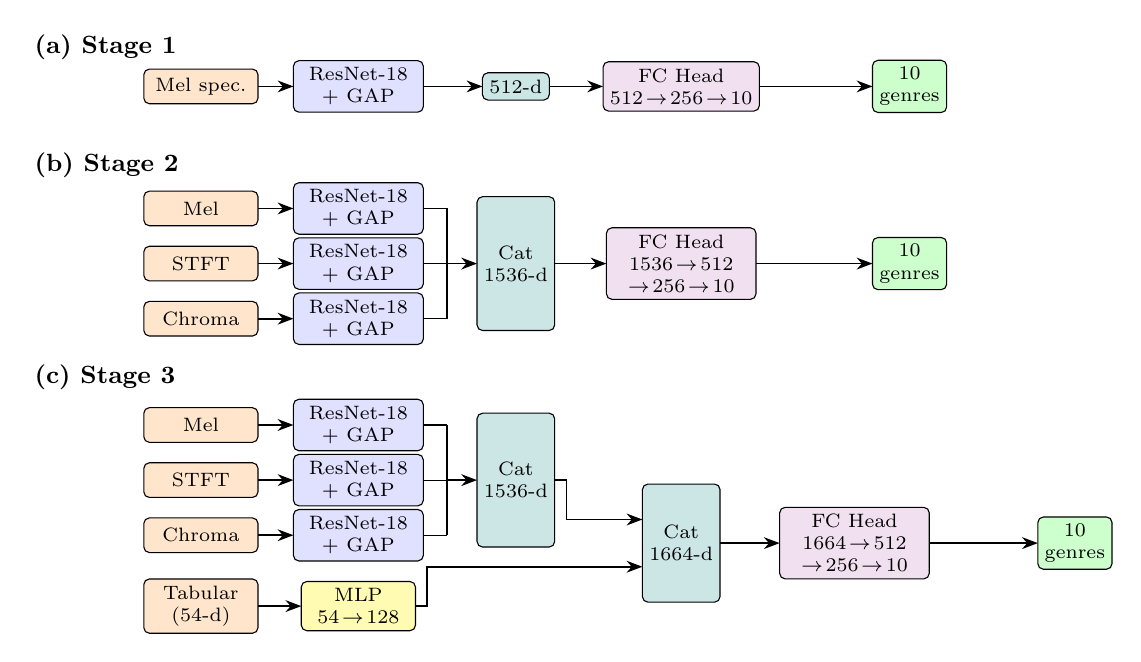
\begin{tikzpicture}[
  every node/.append style={inner sep=2.5pt, outer sep=0pt},
  inp/.style={draw, rounded corners=2pt, fill=orange!20, minimum width=1.45cm, minimum height=0.44cm, align=center, font=\scriptsize},
  cnn/.style={draw, rounded corners=2pt, fill=blue!12,   minimum width=1.65cm, minimum height=0.44cm, align=center, font=\scriptsize},
  mlp/.style={draw, rounded corners=2pt, fill=yellow!30, minimum width=1.45cm, minimum height=0.44cm, align=center, font=\scriptsize},
  cat/.style={draw, rounded corners=2pt, fill=teal!20,   minimum width=0.85cm, align=center, font=\scriptsize},
  hd/.style ={draw, rounded corners=2pt, fill=violet!12, minimum width=1.9cm,  align=center, font=\scriptsize},
  outp/.style={draw, rounded corners=2pt, fill=green!20,  minimum width=0.9cm,  minimum height=0.44cm, align=center, font=\scriptsize},
  arr/.style={-Stealth, semithick},
  stg/.style={font=\small\bfseries, anchor=west},
]

%% ─── Stage 1: label above, single row at y=0 ────────────────────────────────
\node[stg]  at (0,  0.50) {(a)~Stage~1};
\node[inp]  (i1)  at (2.2,  0.00) {Mel spec.};
\node[cnn]  (r1)  at (4.2,  0.00) {ResNet-18\\+~GAP};
\node[cat]  (e1)  at (6.2,  0.00) {512-d};
\node[hd]   (h1)  at (8.3,  0.00) {FC~Head\\$512\!\to\!256\!\to\!10$};
\node[outp] (o1)  at (11.2, 0.00) {10\\genres};
\draw[arr] (i1) -- (r1);
\draw[arr] (r1) -- (e1);
\draw[arr] (e1) -- (h1);
\draw[arr] (h1) -- (o1);

%% ─── Stage 2: label above, rows at y=-1.55, -2.25, -2.95 ───────────────────
\node[stg]  at (0, -1.00) {(b)~Stage~2};
\node[inp]  (i2m) at (2.2, -1.55) {Mel};
\node[inp]  (i2s) at (2.2, -2.25) {STFT};
\node[inp]  (i2c) at (2.2, -2.95) {Chroma};
\node[cnn]  (r2m) at (4.2, -1.55) {ResNet-18\\+~GAP};
\node[cnn]  (r2s) at (4.2, -2.25) {ResNet-18\\+~GAP};
\node[cnn]  (r2c) at (4.2, -2.95) {ResNet-18\\+~GAP};
\draw[arr] (i2m) -- (r2m);
\draw[arr] (i2s) -- (r2s);
\draw[arr] (i2c) -- (r2c);
\coordinate (p2m) at ($(r2m.east)+(0.30,0)$);
\coordinate (p2s) at ($(r2s.east)+(0.30,0)$);
\coordinate (p2c) at ($(r2c.east)+(0.30,0)$);
\draw (r2m.east) -- (p2m);
\draw (r2s.east) -- (p2s);
\draw (r2c.east) -- (p2c);
\draw (p2m) -- (p2c);
\node[cat, minimum height=1.70cm] (cat2) at (6.2, -2.25) {Cat\\1536-d};
\node[hd]   (h2)  at (8.3,  -2.25) {FC~Head\\$1536\!\to\!512$\\$\to\!256\!\to\!10$};
\node[outp] (o2)  at (11.2, -2.25) {10\\genres};
\draw[arr] (p2s) -- (cat2.west);
\draw[arr] (cat2.east) -- (h2.west);
\draw[arr] (h2.east)   -- (o2.west);

%% ─── Stage 3: label above, rows at y=-4.30, -5.00, -5.70, -6.60 ─────────────
\node[stg]  at (0, -3.70) {(c)~Stage~3};
\node[inp]  (i3m) at (2.2, -4.30) {Mel};
\node[inp]  (i3s) at (2.2, -5.00) {STFT};
\node[inp]  (i3c) at (2.2, -5.70) {Chroma};
\node[inp]  (i3t) at (2.2, -6.60) {Tabular\\(54-d)};
\node[cnn]  (r3m) at (4.2, -4.30) {ResNet-18\\+~GAP};
\node[cnn]  (r3s) at (4.2, -5.00) {ResNet-18\\+~GAP};
\node[cnn]  (r3c) at (4.2, -5.70) {ResNet-18\\+~GAP};
\node[mlp]  (m3)  at (4.2, -6.60) {MLP\\$54\!\to\!128$};
\draw[arr] (i3m) -- (r3m);
\draw[arr] (i3s) -- (r3s);
\draw[arr] (i3c) -- (r3c);
\draw[arr] (i3t) -- (m3);
\coordinate (p3m) at ($(r3m.east)+(0.30,0)$);
\coordinate (p3s) at ($(r3s.east)+(0.30,0)$);
\coordinate (p3c) at ($(r3c.east)+(0.30,0)$);
\draw (r3m.east) -- (p3m);
\draw (r3s.east) -- (p3s);
\draw (r3c.east) -- (p3c);
\draw (p3m) -- (p3c);
\node[cat, minimum height=1.70cm] (ca3) at (6.2, -5.00) {Cat\\1536-d};
\draw[arr] (p3s) -- (ca3.west);
\node[cat, minimum height=1.50cm] (cb3) at (8.3, -5.80) {Cat\\1664-d};
\draw[arr] (ca3.east) -- ++(0.15,0) |- ([yshift= 0.30cm]cb3.west);
\draw[arr] (m3.east)  -- ++(0.15,0) |- ([yshift=-0.30cm]cb3.west);
\node[hd]   (h3)  at (10.5, -5.80) {FC~Head\\$1664\!\to\!512$\\$\to\!256\!\to\!10$};
\node[outp] (o3)  at (13.3, -5.80) {10\\genres};
\draw[arr] (cb3.east) -- (h3.west);
\draw[arr] (h3.east)  -- (o3.west);

\end{tikzpicture}%
}
\caption{Architecture overview of the three model stages. \textbf{(a)} Stage~1: single ResNet-18 branch on mel spectrograms. \textbf{(b)} Stage~2: three parallel branches (mel, STFT, chroma) concatenated into a 1536-d joint embedding before a shared FC head. \textbf{(c)} Stage~3: same three CNN branches plus a tabular MLP branch; CNN embeddings are first concatenated (1536-d), then concatenated with the 128-d tabular embedding (1664-d total) before the FC head. Colours: orange = input, blue = ResNet-18+GAP, yellow = tabular MLP, teal = concatenation, purple = FC head, green = output.}
\label{fig:arch_stages}
\end{figure*}

\subsection{Backbone and Training Protocol}

Figure~\ref{fig:arch_stages} gives an overview of all three stages. All CNN branches use \textbf{ResNet-18} \cite{he2016} as the feature extraction backbone, initialised with ImageNet pretrained weights. ResNet-18 is chosen for three reasons: (1) it is compact enough to train multiple parallel copies within GPU memory constraints; (2) Palanisamy~et~al.~\cite{palanisamy2020} demonstrate that ImageNet-pretrained ResNets are strong baselines for audio classification with spectrogram inputs; and (3) the GTZAN training set ($\approx$7,900 segments before augmentation) is too small to train a deep network from random initialisation without severe overfitting.

The standard 1,000-class FC head is replaced with a task-specific classification head for each stage. The Global Average Pooling (GAP) layer that reduces the final $4\times4\times512$ feature map to a 512-d vector serves as the branch embedding output. Layer-by-layer dimensions are detailed in Appendix~\ref{app:arch}.

\textbf{Transfer learning and progressive unfreezing.} Despite the domain shift from natural images to plasma-colourised spectrograms, early ResNet layers learn general edge and texture detectors that transfer well to time-frequency representations. To avoid destroying pretrained representations early in training, a progressive unfreezing schedule is adopted: layers 1--3 are frozen for the first 4 epochs (head-only training, lr\,$=10^{-3}$), then \texttt{layer4} is unfrozen at epoch 5 with a reduced backbone lr\,$=10^{-4}$, allowing high-level feature adaptation while lower layers remain stable.

\textbf{Optimiser and regularisation.} All models are trained with Adam \cite{kingma2014} ($\beta_1=0.9$, $\beta_2=0.999$), a StepLR scheduler ($\gamma=0.5$, step 10 epochs), and early stopping on validation loss (patience 7). At every epoch, model weights achieving the best validation accuracy are checkpointed and restored at the end of training. Full hyperparameters are listed in Appendix~\ref{app:arch}.

\subsection{Stage 1: Single-Branch Mel Baseline}

Stage 1 establishes a single-modality baseline using mel spectrograms as the sole CNN input. The classification head appended after the 512-d GAP embedding is: FC(512$\to$256)+ReLU, Dropout(0.4), FC(256$\to$10). The intermediate 256-d hidden layer introduces a non-linear bottleneck; dropout with $p=0.4$ provides regularisation appropriate for the dataset size. Head-only trainable parameters: $(512\times256+256)+(256\times10+10)=133{,}898$.

\subsection{Stage 2: Three-Branch Fusion}

Stage 2 extends Stage 1 by processing all three spectral representations in parallel. Three independent ResNet-18 branches (mel, STFT, chroma) each produce 512-d embeddings via GAP, which are concatenated into a 1,536-d joint representation and passed through a shared fusion head: FC(1536$\to$512)+ReLU, Dropout(0.4), FC(512$\to$256)+ReLU, Dropout(0.3), FC(256$\to$10).

The two-stage compression (1,536$\to$512$\to$256) allows cross-modal interactions to be learned at multiple levels of abstraction. The three modalities are chosen to provide \textbf{complementary information}: mel captures perceptual timbre; STFT retains high-frequency spectral detail that mel's logarithmic compression discards; and chroma encodes harmonic/chord vocabulary largely absent from mel spectrograms \cite{wolfmonheim2024, zhang2025}. The batch size is reduced to 32 (from 64 in Stage 1) to accommodate the tripled memory footprint of loading three spectrograms per sample. Each branch's \texttt{layer4} is unfrozen simultaneously at epoch 5.

\subsection{Stage 3: CNN Fusion with Tabular Branch}

Stage 3 adds a fourth branch: a two-layer MLP (FC(54$\to$128)+ReLU, Dropout(0.4)) that maps the 54 standardised tabular features to a 128-d embedding. The 128-d tabular embedding is \textit{directly concatenated} with the 1,536-d CNN embedding, without first compressing the CNN representation. This design allows the joint FC head (FC(1664$\to$512)+ReLU, Dropout(0.4), FC(512$\to$256)+ReLU, Dropout(0.3), FC(256$\to$10)) to learn the optimal compression of both modalities jointly, enabling it to discover interactions between CNN and tabular features rather than forcing them into separate bottlenecks.

The hypothesis is that hand-crafted MIR features accumulated through decades of domain expertise \cite{tzanetakis2002} encode complementary global statistics (tempo, MFCC cepstral coefficients, zero-crossing rate, RMS) that convolutional operations on local spectrogram patches may not fully capture. Projecting first to 128 dimensions (slightly larger than the 54-d input) allows the MLP to learn non-linear feature interactions before fusion.

% =============================================================================
\section{Evaluation}
% =============================================================================

\subsection{Experimental Setup}

All three stages are evaluated on the held-out test split of 990 three-second segments (99 tracks, $\approx$10 per genre), which was never used during training or hyperparameter selection. The primary metric is top-1 accuracy: the fraction of test segments for which the model's argmax prediction matches the ground-truth label. For each stage, the weights restored at the end of training are the best-val-accuracy checkpoint.

\subsection{Results}

Table~\ref{tab:results} shows that each additional stage yields a consistent improvement. Stage 1$\to$2 gains $+2.83$ pp by adding STFT and chroma branches, confirming that the two additional modalities provide complementary discriminative signal beyond mel alone. Stage 2$\to$3 gains a further $+2.32$ pp by adding the tabular MLP branch, confirming that hand-crafted MIR statistics encode information not captured by the CNN branches. The consistent monotonic improvement across stages validates each architectural hypothesis.

\begin{table}[H]
\centering
\caption{Test-set accuracy for each model stage.}
\label{tab:results}
\resizebox{\columnwidth}{!}{%
\begin{tabular}{llr}
\toprule
\textbf{Stage} & \textbf{Architecture} & \textbf{Test Acc.} \\
\midrule
Stage 1 & Single-branch ResNet-18 (mel) & 75.96\% \\
Stage 2 & Three-branch CNN fusion & 78.79\% \\
Stage 3 & CNN fusion + tabular MLP & \textbf{81.11\%} \\
\bottomrule
\end{tabular}%
}
\end{table}

\subsection{Per-Class Analysis}

Table~\ref{tab:perclass} reports the Stage 3 per-genre classification report and Figure~\ref{fig:confusion} shows the full confusion matrix. \textbf{Classical} (F1\,=\,0.94) and \textbf{jazz} (F1\,=\,0.90) are the best-performing genres. Classical benefits from its highly distinctive orchestral timbres and lack of percussion, making it a near-isolated cluster in feature space (visible in the PCA plot, Appendix~\ref{app:eda}). Jazz scores well due to its complex harmonic vocabulary, which the chroma branch captures effectively.

\textbf{Pop} and \textbf{rock} are the most challenging (F1\,=\,0.67 each). Rock is frequently misclassified as blues or country, which share guitar-dominant timbres and similar rhythmic structures. Pop is confused with country and disco, reflecting overlapping production styles and rhythmic templates across these commercially adjacent genres. \textbf{Disco} (F1\,=\,0.71) also suffers from its rhythmic overlap with hip-hop and its stylistic closeness to pop. This is unsurprising, considering that even human annotators disagree at genre boundaries, and the 30-second clips further reduce the available acoustic context.

\begin{table}[H]
\centering
\caption{Per-genre classification report, Stage 3 (test set, $n=990$).}
\label{tab:perclass}
\begin{tabular}{lccc}
\toprule
\textbf{Genre} & \textbf{Prec.} & \textbf{Recall} & \textbf{F1} \\
\midrule
Blues      & 0.81 & 0.91 & 0.85 \\
Classical  & 0.93 & 0.94 & 0.94 \\
Country    & 0.79 & 0.82 & 0.80 \\
Disco      & 0.72 & 0.70 & 0.71 \\
Hip-hop    & 0.89 & 0.78 & 0.83 \\
Jazz       & 0.95 & 0.86 & 0.90 \\
Metal      & 0.82 & 0.91 & 0.86 \\
Pop        & 0.66 & 0.69 & 0.67 \\
Reggae     & 0.87 & 0.88 & 0.88 \\
Rock       & 0.71 & 0.63 & 0.67 \\
\midrule
\textbf{Macro avg} & \textbf{0.81} & \textbf{0.81} & \textbf{0.81} \\
\bottomrule
\end{tabular}
\end{table}

\begin{figure*}[t]
    \centering
    
\includegraphics[width=0.7\textwidth]{figures/stage3_confusion.pdf}
    \caption{Confusion matrix for the Stage 3 model on the 990-segment test set (raw segment counts). Rows are true labels; columns are predicted labels.}
    \label{fig:confusion}
\end{figure*}

\subsection{Comparison with Baseline}

The reference baseline is the most upvoted Kaggle notebook by Olteanu \cite{olteanu2020} (the author who compiled the GTZAN dataset on Kaggle), which trains classical ML classifiers on tabular features. Table~\ref{tab:baseline} compares all baselines against the proposed stages. XGBoost achieves a headline 90.22\%, outperforming our best Stage 3 model by 9.11 pp.

\begin{table}[H]
\centering
\caption{Tabular ML baselines \cite{olteanu2020} vs.\ proposed CNN stages.}
\label{tab:baseline}
\resizebox{\columnwidth}{!}{%
\begin{tabular}{llr}
\toprule
\textbf{Model} & \textbf{Input} & \textbf{Acc.} \\
\midrule
Naive Bayes          & Tabular & 51.95\% \\
SGD Classifier       & Tabular & 65.53\% \\
Decision Tree        & Tabular & 64.00\% \\
Logistic Regression  & Tabular & 69.77\% \\
MLP (shallow)        & Tabular & 67.73\% \\
SVM (RBF)            & Tabular & 75.41\% \\
KNN                  & Tabular & 80.58\% \\
XGBoost (RF mode)    & Tabular & 74.88\% \\
\textbf{XGBoost}     & \textbf{Tabular} & \textbf{90.22\%} \\
\midrule
Stage 1 (ours) & Mel spectrogram & 75.96\% \\
Stage 2 (ours) & Mel+STFT+chroma & 78.79\% \\
Stage 3 (ours) & Images+tabular  & \textbf{81.11\%} \\
\bottomrule
\end{tabular}%
}
\end{table}

\subsection{Discussion}

\paragraph{Data leakage in the baseline.}
The 9.11 pp gap between Stage 3 and XGBoost is partly a methodological artefact of two data leakages in the baseline. \textbf{Leakage 1}: the baseline applies \texttt{train\_test\_split} directly to the 9,990-row segment dataframe, so segments from the same track appear in both train and test. Because segments from the same 30-second recording are acoustically near-identical, the model effectively memorises tracks rather than learning genre-discriminative features \cite{sturm2013}. \textbf{Leakage 2}: \texttt{MinMaxScaler.fit\_transform} is called on the full 9,990-row dataframe before splitting, contaminating the scaler with test-set statistics. Both leakages inflate the reported accuracy. Our strict track-level protocol produces a harder but methodologically sound evaluation.

\paragraph{Inherent advantages of the tabular baseline.}
Beyond leakage, XGBoost benefits from two structural advantages. First, the MIR tabular features are \textit{expert-designed} to be genre-discriminative (tempo, MFCCs, spectral shape) and directly encode domain knowledge accumulated over decades. Second, the GTZAN dataset's small size (988 tracks) structurally favours low-dimensional tree-based models: gradient-boosted trees require far fewer samples to generalise than a three-branch CNN with millions of parameters, even with transfer learning and aggressive augmentation.

\paragraph{Directions for improvement.}
Several directions could close the remaining gap. \textbf{Test-time aggregation} (majority or soft vote across the 10 segments of each track) would boost accuracy at inference time with no additional training cost, since track-level predictions are more stable than individual 3-second segment predictions. \textbf{Audio-domain pretraining} via VGGish \cite{hershey2017} or PANNs \cite{kong2020} would replace ImageNet priors with representations pre-trained on millions of audio clips, better suited to spectro-temporal patterns. \textbf{Systematic hyperparameter search} (learning rate, dropout rates, FC widths, MLP depth, augmentation strengths) was not performed due to compute constraints and could yield meaningful gains across all stages.

% =============================================================================
\section{Conclusion}
% =============================================================================

This work demonstrates that progressively richer fusion of acoustic representations yields consistent accuracy gains on GTZAN: Stage 1 (single-branch mel, 75.96\%) $\to$ Stage 2 (three-branch fusion, 78.79\%) $\to$ Stage 3 (CNN+tabular, 81.11\%). Each architectural addition validates its underlying hypothesis: STFT and chroma branches provide complementary spectral and harmonic information, and hand-crafted MIR statistics provide global segment-level cues not fully captured by local convolutional operations.

The 9.11 pp gap to the XGBoost tabular baseline (90.22\%) is partly a methodological artefact: the baseline uses segment-level splitting and pre-split feature scaling, both of which inflate its reported accuracy. On a fair evaluation, the advantage of expert-designed tabular features over ImageNet-pretrained CNNs on a 988-track dataset is expected and reflects the structural advantage of gradient-boosted trees on small, low-dimensional feature matrices.

Closing the gap fully would likely require moving beyond GTZAN's constraints: audio-domain pretraining (VGGish \cite{hershey2017}, PANNs \cite{kong2020}), track-level inference aggregation, or end-to-end waveform learning. The staged fusion architecture developed here nonetheless provides a reusable blueprint for multimodal audio classification under data-scarce conditions, with each modality's contribution cleanly isolated and empirically validated.

% =============================================================================
\bibliographystyle{IEEEtran}
\bibliography{references_shortened}

% =============================================================================
\appendix

% =============================================================================
\section{Mathematical Foundations of Acoustic Representations}
\label{app:math}
% =============================================================================

\paragraph{Discrete Fourier Transform.}
A digital audio signal is a discrete sequence of air pressure measurements sampled at rate $f_s$. The \textbf{Discrete Fourier Transform (DFT)} decomposes a finite-length signal $x[n]$ of length $N$ into its constituent complex sinusoids \cite{oppenheim2010}:
\[
    X[k] = \sum_{n=0}^{N-1} x[n] \cdot e^{-j 2\pi k n / N}, \quad k = 0, \ldots, N-1
\]
where $X[k]$ is the complex amplitude of frequency $f_k = k f_s / N$. The magnitude $|X[k]|$ indicates how strongly that frequency is present. The FFT computes this in $O(N \log N)$ \cite{cooley1965}.

\paragraph{Short-Time Fourier Transform.}
Music is non-stationary, so the DFT of an entire track discards temporal structure. The \textbf{STFT} computes the DFT over short, overlapping windows \cite{allen1977}:
\[
    \mathbf{S}[m, k] = \sum_{n=0}^{N_{\text{fft}}-1} x[n + m H] \cdot w[n] \cdot e^{-j 2\pi k n / N_{\text{fft}}}
\]
where $m$ is the frame index, $H$ is the hop length, and $w[n]$ is a Hann window that reduces spectral leakage. The power spectrogram $|\mathbf{S}[m,k]|^2$ is converted to dB:
\[
    \mathbf{S}_{\text{dB}}[m, k] = 10 \log_{10}\!\left( |\mathbf{S}[m, k]|^2 \right) - 10 \log_{10}\!\left( \max_{m,k} |\mathbf{S}[m, k]|^2 \right)
\]
compressing the dynamic range to roughly $[-80, 0]$ dB. Parameters used: $N_{\text{fft}}=2048$, $H=512$, $f_s=22{,}050$ Hz, yielding $\approx$130 time frames and 1,025 frequency bins per 3-second segment.

\paragraph{Mel Spectrogram.}
Human pitch perception is logarithmic in frequency. The \textit{mel scale} models this \cite{oshaughnessy1987}:
\[
    m(f) = 2595 \cdot \log_{10}\!\left(1 + \frac{f}{700}\right)
\]
A bank of $M_{\text{mel}}=128$ triangular filters, uniformly spaced on the mel axis, is applied to the STFT power spectrum \cite{davis1980}:
\[
    \mathbf{M}[m, l] = \sum_{k} \mathbf{H}_l[k] \cdot |\mathbf{S}[m, k]|^2, \quad l = 1, \ldots, 128
\]
giving a $128 \times 130$ representation that captures perceptual timbre. Wolf-Monheim \cite{wolfmonheim2024} show mel spectrograms substantially outperform other single representations for audio CNN classification.

\paragraph{Chromagram.}
A \textbf{chromagram} projects the spectrum onto the 12 pitch classes of the Western chromatic scale by summing energy across all octaves \cite{muller2015}:
\[
    \mathbf{C}[m, p] = \sum_{k:\, \text{pitch}(f_k) = p} |\mathbf{S}[m, k]|^2, \quad p \in \{0, \ldots, 11\}
\]
The resulting $12 \times M$ matrix captures harmonic and tonal structure, strongly discriminating genres by chord vocabulary (e.g., jazz complex chords vs.\ metal power chords).

\begin{table}[H]
\centering
\caption{Summary of the three CNN input representations.}
\resizebox{\columnwidth}{!}{%
\begin{tabular}{llll}
\toprule
\textbf{Representation} & \textbf{Axes} & \textbf{Raw shape} & \textbf{Captures} \\
\midrule
STFT Spectrogram & Time $\times$ Freq.\ (linear) & $1025 \times 130$ & Full spectral content \\
Mel Spectrogram  & Time $\times$ Freq.\ (mel)    & $128 \times 130$  & Perceptual timbre \\
Chromagram       & Time $\times$ Pitch class     & $12 \times 130$   & Harmonic/tonal content \\
\bottomrule
\end{tabular}%
}
\end{table}

% =============================================================================
\section{Exploratory Data Analysis}
\label{app:eda}
% =============================================================================

\paragraph{Feature Distributions.}
Kernel density estimates of six representative tabular features (Figure~\ref{fig:feature_dist_app}) confirm that no single feature cleanly separates all 10 genres. Tempo discriminates fast-paced genres (metal, disco) from slower ones (blues, classical); spectral centroid is elevated for high-energy genres (pop, metal); zero-crossing rate is highest for percussive and distorted genres.

\begin{figure}[H]
    \centering
    
\includegraphics[width=\columnwidth]{figures/feature_distributions.pdf}
    \caption{Kernel density estimates of six representative features across 10 genres (3-second segments). Overlapping distributions indicate no single feature is sufficient for reliable genre separation.}
    \label{fig:feature_dist_app}
\end{figure}

\paragraph{Feature Correlation Analysis.}
Pairwise Pearson correlations among the 57 numerical features reveal four highly correlated pairs ($|r| \geq 0.90$), listed in Table~\ref{tab:corr_pairs}. \texttt{rolloff\_mean} appears in three of the four pairs; together with \texttt{spectral\_\allowbreak bandwidth\_mean} and \texttt{spectral\_\allowbreak centroid\_mean} it is dropped, retaining \texttt{mfcc2\_mean} as it is empirically the most discriminative feature group \cite{tzanetakis2002}. This reduces feature dimensionality from 57 to 54.

\begin{table}[H]
\centering
\caption{Highly correlated feature pairs ($|r| \geq 0.90$).}
\label{tab:corr_pairs}
\resizebox{\columnwidth}{!}{%
\begin{tabular}{llc}
\toprule
\textbf{Feature 1} & \textbf{Feature 2} & \textbf{Corr.} \\
\midrule
\texttt{spectral\_centroid\_mean}   & \texttt{rolloff\_mean}            & $+0.974$ \\
\texttt{spectral\_bandwidth\_mean}  & \texttt{rolloff\_mean}            & $+0.951$ \\
\texttt{spectral\_centroid\_mean}   & \texttt{mfcc2\_mean}              & $-0.931$ \\
\texttt{rolloff\_mean}              & \texttt{mfcc2\_mean}              & $-0.923$ \\
\bottomrule
\end{tabular}%
}
\end{table}

\begin{figure}[H]
    \centering
    
\includegraphics[width=\columnwidth]{figures/correlation_heatmap.pdf}
    \caption{Pairwise Pearson correlation matrix of the 57 numerical features.}
    \label{fig:corr_heatmap_app}
\end{figure}

\paragraph{PCA Visualisation and Outlier Detection.}
PCA on the standardised 57-feature matrix yields a 2D projection explaining $\approx$33.6\% of variance. The projection (Figure~\ref{fig:pca_app}) shows heavy genre entanglement, motivating non-linear models. Outliers are segments whose Euclidean distance from their genre centroid in PCA space exceeds $3\sigma$; tracks with $\geq 8$ outlier segments out of 10 are flagged as track-level anomalies and removed during cleaning.

\begin{figure}[H]
    \centering
    
\includegraphics[width=\columnwidth]{figures/pca_scatter.pdf}
    \caption{2D PCA projection (standardised features). Left: genre clusters. Right: outlier segments ($>3\sigma$ from genre centroid) highlighted. Classical forms the most compact cluster; rock, country, and blues overlap heavily.}
    \label{fig:pca_app}
\end{figure}

% =============================================================================
\section{Detailed Model Architectures and Hyperparameters}
\label{app:arch}
% =============================================================================

\begin{table}[H]
\centering
\caption{ResNet-18 layer-by-layer output dimensions for a $128\times128\times3$ input.}
\resizebox{\columnwidth}{!}{%
\begin{tabular}{lll}
\toprule
\textbf{Stage} & \textbf{Output shape} & \textbf{Description} \\
\midrule
Input                  & $128\times128\times3$ & RGB spectrogram \\
Stem (Conv1+MaxPool)   & $32\times32\times64$  & $7\times7$ conv stride 2; $3\times3$ maxpool stride 2 \\
Layer 1                & $32\times32\times64$  & $2\times$ BasicBlock, 64 ch \\
Layer 2                & $16\times16\times128$ & $2\times$ BasicBlock, 128 ch, stride 2 \\
Layer 3                & $8\times8\times256$   & $2\times$ BasicBlock, 256 ch, stride 2 \\
Layer 4                & $4\times4\times512$   & $2\times$ BasicBlock, 512 ch, stride 2 \\
GAP                    & 512                   & Global Average Pooling \\
\bottomrule
\end{tabular}%
}
\end{table}

\begin{table}[H]
\centering
\caption{Training hyperparameters, common across all stages unless noted.}
\resizebox{\columnwidth}{!}{%
\begin{tabular}{lll}
\toprule
\textbf{Hyperparameter} & \textbf{Value} & \textbf{Notes} \\
\midrule
Optimiser                        & Adam       & $\beta_1{=}0.9$, $\beta_2{=}0.999$, $\varepsilon{=}10^{-8}$ \cite{kingma2014} \\
Loss function                    & Cross-entropy & Standard multi-class \\
Head LR                          & $10^{-3}$  & Epochs 1+ \\
Backbone LR (\texttt{layer4})    & $10^{-4}$  & From epoch 5 \\
LR scheduler                     & StepLR     & Step 10, $\gamma=0.5$ \\
Unfreeze epoch                   & 5          & \texttt{layer4} added at epoch 5 \\
Max epochs                       & 30         & Hard limit \\
Early stopping patience          & 7 epochs   & Monitors val.\ loss \\
Best-weight criterion            & Max val.\ acc & Checkpoint restored at end \\
Batch size (Stage 1)             & 64         & Single spectrogram/sample \\
Batch size (Stages 2 \& 3)       & 32         & Three spectrograms/sample \\
Dropout (first FC)               & 0.4        & All heads \\
Dropout (second FC)              & 0.3        & Stages 2 \& 3 only \\
Random seed                      & 42         & \texttt{torch} and \texttt{numpy} \\
\bottomrule
\end{tabular}%
}
\end{table}

\begin{table}[H]
\centering
\caption{Stage 1 architecture (single-branch mel baseline).}
\resizebox{\columnwidth}{!}{%
\begin{tabular}{lll}
\toprule
\textbf{Layer} & \textbf{Output dim} & \textbf{Notes} \\
\midrule
Input (mel spectrogram)    & $128\times128\times3$ & Plasma-colourised, ImageNet-normalised \\
ResNet-18 + GAP            & 512 & Pretrained; layers 1--3 frozen \\
FC(512$\to$256) + ReLU     & 256 & \\
Dropout(0.4)               & 256 & \\
FC(256$\to$10)             & 10  & Genre logits \\
\bottomrule
\end{tabular}%
}
\end{table}

\begin{table}[H]
\centering
\caption{Stage 2 architecture (three-branch CNN fusion).}
\resizebox{\columnwidth}{!}{%
\begin{tabular}{lll}
\toprule
\textbf{Layer} & \textbf{Output dim} & \textbf{Notes} \\
\midrule
Mel / STFT / Chroma ResNet-18 + GAP & $3\times512$ & Pretrained; layers 1--3 frozen \\
Concatenation                        & 1536 & $512\times3$ joint embedding \\
FC(1536$\to$512) + ReLU              & 512  & \\
Dropout(0.4)                         & 512  & \\
FC(512$\to$256) + ReLU               & 256  & \\
Dropout(0.3)                         & 256  & \\
FC(256$\to$10)                       & 10   & Genre logits \\
\bottomrule
\end{tabular}%
}
\end{table}

\begin{table}[H]
\centering
\caption{Stage 3 architecture (CNN fusion + tabular MLP branch).}
\resizebox{\columnwidth}{!}{%
\begin{tabular}{lll}
\toprule
\textbf{Layer} & \textbf{Output dim} & \textbf{Notes} \\
\midrule
Mel / STFT / Chroma ResNet-18 + GAP & $3\times512$ & \\
Concatenation (CNN)                  & 1536 & \\
\midrule
Tabular input                        & 54   & Standardised \\
FC(54$\to$128) + ReLU                & 128  & \\
Dropout(0.4)                         & 128  & \\
\midrule
Concatenation (CNN + tabular)        & 1664 & $1536+128$ \\
FC(1664$\to$512) + ReLU              & 512  & \\
Dropout(0.4)                         & 512  & \\
FC(512$\to$256) + ReLU               & 256  & \\
Dropout(0.3)                         & 256  & \\
FC(256$\to$10)                       & 10   & Genre logits \\
\bottomrule
\end{tabular}%
}
\end{table}

% =============================================================================
\section{Dataset Size at Each Processing Stage}
\label{app:dataset}
% =============================================================================

\begin{table}[H]
\centering
\caption{Segment counts after cleaning and augmentation.}
\resizebox{\columnwidth}{!}{%
\begin{tabular}{lrrrr}
\toprule
\textbf{Split} & \textbf{Orig.} & \textbf{Aug.} & \textbf{Total segs} & \textbf{Images} \\
\midrule
Train & 7{,}891  & 31{,}564 & 39{,}455 & 118{,}365 \\
Val   &    990  &       0  &    990   &   2{,}970 \\
Test  &    990  &       0  &    990   &   2{,}970 \\
\midrule
\textbf{Total} & \textbf{9{,}871} & \textbf{31{,}564} & \textbf{41{,}435} & \textbf{124{,}305} \\
\bottomrule
\end{tabular}%
}
\end{table}

\end{document}
